% !TeX root = ../libro.tex
% !TeX encoding = utf8

\chapter{Estudio de la teselación}

En este capítulo se describe el estudio realizado para teselar de manera eficiente un triángulo. Esta técnica se implementará en shaders, para poder ejecutarlo directamente en la GPU, que ofrece mayor rendimiento que la CPU para dicho problema. En un principio se iba a realizar en un Geometry Shader pero más tarde se observó que era más acertado el uso de un Tessellation Shader. \\
\\ Cabe destacar antes que la idea inicial era desarrollar un algoritmo de división recursiva de los triángulos, el cuál se detiene en el nivel en el que se cree que representa correctamente a la porción de superficie. Sin embargo, el lenguaje Glsl no permite realizar llamadas recursivas, por lo que era necesario buscar alternativas.

\section{Geometry shader}
	La ventaja de este tipo de shader es que es muy flexible a la hora de generar nuevas primitivas, ya que permite añadir primitivas totalmente disconexas.\\
	\\ En primer lugar opté por describir de forma explícita un cierto número de niveles de la función recursiva deseada, $3$ niveles concretamente. Los resultados eran aceptables pero se podía exceder el límite de vértices, quedando así una superficie incompleta. Además, el tiempo de compilación crecía de forma exponencial a medida que se añadían más niveles (para $2$ niveles era de $10$-$15$s y para $3$ no concluía).\\
	\\ Puesto que este método era costoso temporalmente y tenía muchas limitaciones, decidí implementar un algoritmo similar pero en un bucle, cuyo esquema es el siguiente:
	\begin{enumerate}
		\item Dado un lado, dividirlo en tantos segmentos como sea necesario, atendiendo a una cierta medida. Dicha medida sólo depende de las características del lado, para que el pegado sea el correcto con los triángulos adyacentes.
		\item Se realiza una división hacia el baricentro, de forma similar al punto anterior.
		\item Con los vértices de los dos puntos anteriores se genera una malla, es decir, para cada lado, se genera otro lado paralelo para cada subdivisión hacia el baricentro, manteniendo proporcionalmente las subdivisiones del lado original.
		\item Se genera una tira de triángulos cuyos vértices sean los de la malla anterior.
	\end{enumerate}
	
	Con este método los problemas anteriores se solventan en gran medida, pero dicho algoritmo es semejante al del Tessellation shader, por lo que era natural estudiar el funcionamiento en tal shader.\\
	\\ Finalmente, los inconvenientes observados han sido los siguientes:
	\begin{itemize}
		\item El número de vértices de salida está limitado por una constante predefinida, con valor GL$\_$MAX$\_$GEOMETRY$\_$OUTPUT$\_$VERTICES=$256$ (depende del hardware), es decir, como mucho se puede devolver una tira de $254$ triángulos, independientemente del tamaño del triángulo original.
		\item El shader tarda en compilarse de media entre $3$ y $5$ segundos.
	\end{itemize}
	
\section{Tessellation shader}

	Este shader tiene un pequeño problema y es que la subdivisión está predefinida (equal, fractional$\_$odd o fractional$\_$even spacing), por lo que los vértices generados en la fase de control del Tessellation shader tienen un esquema fijo, para un número de subdivisiones dado. No es un gran inconveniente puesto que en la fase de evaluación se pueden variar libremente dichos vértices, siempre que se haga con cuidado (en esta fase los vértices se generan mediante coordenadas baricéntricas). \\
	\\ Las ventajas con respecto al Geometry shader son las siguientes:
	\begin{itemize}
		\item El shader tarda en compilarse de media menos de $1s$.
		\item El número de vértices de salida no está tan limitado (GL$\_$MAX$\_$PATCH$\_$VERTICES$=36477$ frente a $256$).
		\item Está pensado para realizar directamente el algoritmo de teselación, por lo que no hay que implementarlo.
	\end{itemize}
	
	Al tener implementado el algoritmo de teselación, el estudio se reduce a encontrar una medida que nos indique cómo de buena es la representación de la superficie. Como la teselación se indica por cada lado (outer tessellation factor) y en el interior (inner tessellation), para cada tipo de medida hay que proporcionar una adicional para los lados, para que la teselación sólo dependa de lo que sucede en ellos y de esta forma pegue correctamente con el triángulo adyacente.
	
	\subsection{Medida basada en el volumen}
	
	Consiste en estimar el volumen de la diferencia entre el poliedro generado y la superficie original a nivel local. Esta medida está asociada al primer concepto de superficie bien representada:
	\begin{definicion}[Superficie bien representada 1]
		Dada una superficie $S$ y un politopo $P$ que la aproxima, se dice que la representa con una precisión de $\epsilon > 0$ si el volumen contenido entre ambos es menor que $\epsilon$.
	\end{definicion}
	La medida equivalente para los lados es el área de la sección cuya base es el lado del triángulo y el borde restante es la curva original a aproximar con dicho lado.\\ 
	\begin{figure}[h]
  		\centering
  		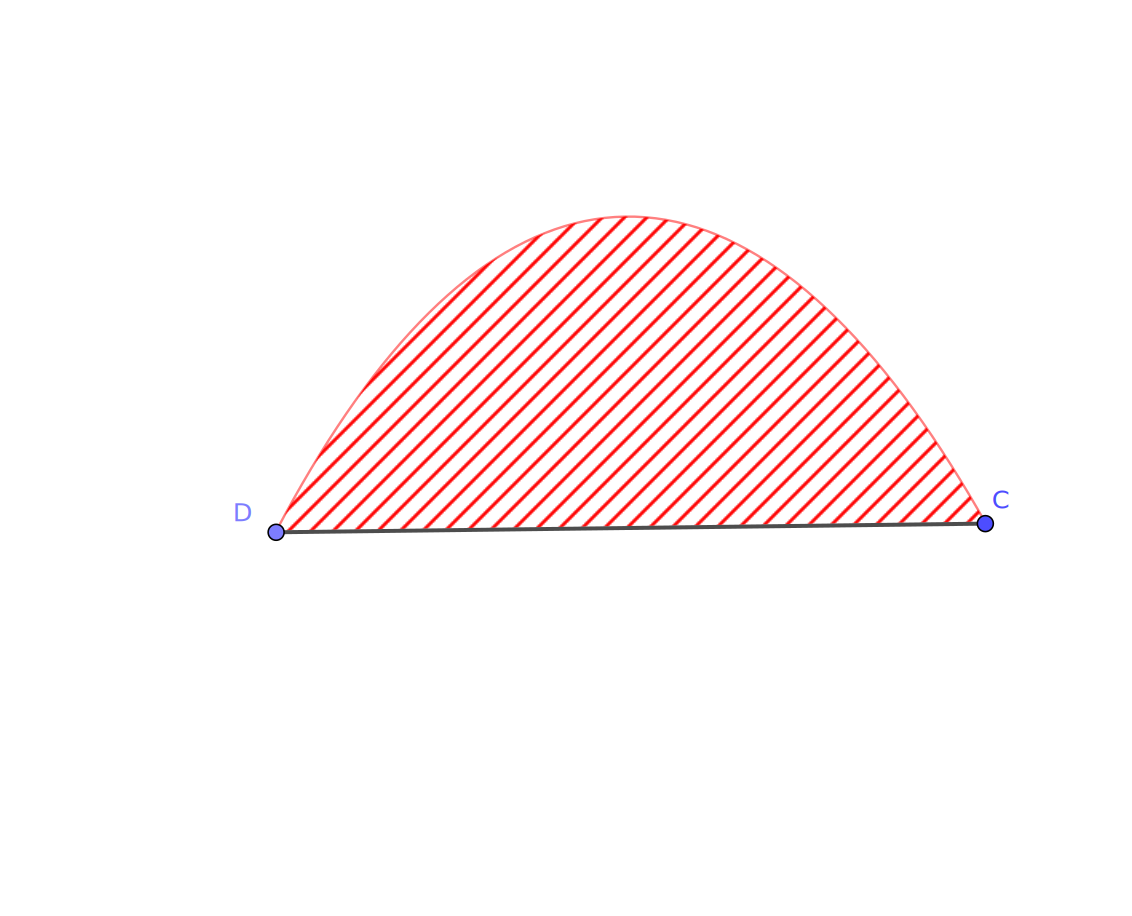
\includegraphics[width=0.5\textwidth]{seccion_area}
  		\caption{Medida en un lado $DC$}
  		\label{fig:seccion_area}
	\end{figure}
	\\ Sin embargo, para las superficies no compactas esta definición puede no permitir la existencia de un $P$ que la aproxime con una precisión finita.\\
	\\ Además, aparece el problema de la no detección de picos, debido a que al estudiar el volumen, si la altura es grande y la base lo suficientemente pequeña se puede dar el caso de que el volumen quede por debajo de la precisión $\epsilon$ y no tesele, aun existiendo dicho pico.
	\begin{figure}[h]
  		\centering
  		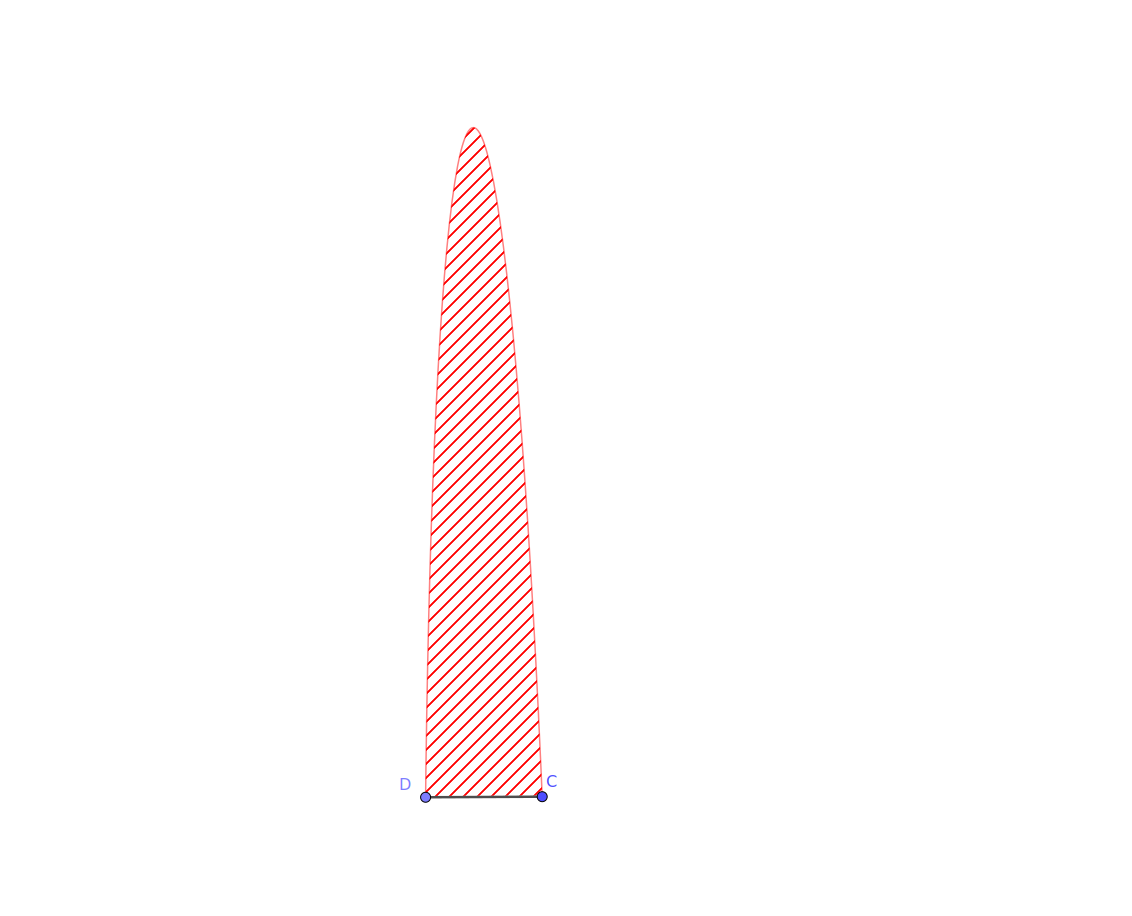
\includegraphics[width=0.6\textwidth]{pico_volumen}
  		\caption{Pico no teselado}
  		\label{fig:pico_volumen}
	\end{figure}
	
	\subsection{Medida basada en el área}
	
	Consiste en estimar el área de la superficie original localmente. Esta medida está asociada al segundo concepto de superficie bien representada:
	\begin{definicion}[Superficie bien representada 2]
		Dada una superficie $S$ y un politopo $P$ que la aproxima, se dice que la representa con una precisión de $\epsilon > 0$ si el ratio de área $r=\frac{A(S)} {A(P)}$ cumple que $r-1 < \epsilon$ (siempre se tiene que $r\geq 1$).
	\end{definicion}
	
	La medida equivalente para los lados es $r=\frac{L(\alpha)} {L(l)}$ donde $L$ es la longitud, $l$ el lado del triángulo y $\alpha$ la curva a estimar.\\
	\\Es una buena alternativa para poder detectar dichos picos, ya que cuando hay uno o varios picos mal aproximados el área original entorno al pico es mucho mayor que la de la superficie generada (el ratio es grande). Además, de esta forma estamos evitando la aparición del problema del farolillo de Schwarz (--CITAR--) debido a que buscamos estimar con una cierta precisión el área original.\\
	\\Sin embargo, al usar esta medida asumimos que la parametrización a nivel local funciona como una gráfica, como por ejemplo $p(u,v)=(p_x(u,v),p_y(u,v),p_z(u,v)) = (u,v,p_z(u,v))$. Esto no es cierto en la gran mayoría de casos y se puede ver fácilmente con la siguiente parametrización del plano $[0,1]x[0,1]$, embebido en $\R^3$:
	$$p(u,v)=(cos(\frac{\pi}{2} u), sin(\frac{\pi}{2} v), 0 )$$
	\\Al ser un plano no debería de teselar, pero como detecta que la curva a estimar en el lado del triángulo no está bien aproximada, entonces subdivide:
	\begin{figure}[h]
  		\centering
  		\includegraphics[width=0.2\textwidth]{tess_plano_k}
  		\includegraphics[width=0.2\textwidth]{tess_plano_long}
  		\caption{Teselación innecesaria del plano}
  		\label{fig:plano_tess}
	\end{figure}
	
	\subsection{Medida basada en la curvatura}
	Consiste en estimar la curvatura de Gauss por área. Esta medida está asociada al tercer concepto de superficie bien representada:
	\begin{definicion}[Superficie bien representada 3]
		Dada una superficie $S$ y un politopo $P$ que la aproxima, se dice que la representa con una precisión de $\epsilon > 0$ si para todo triángulo $T$ del politopo se cumple que $K_T A(T) < \epsilon$, donde $K_T$ es el máximo valor de la curvatura de Gauss en valor absoluto en $T$.
	\end{definicion}
	
	La medida equivalente para los lados es $K_l L$ donde $L$ es la longitud y $l$ el lado del triángulo.\\
	\\Si utilizamos como medida sólo la curvatura, que no depende de la parametrización de la superficie, teselaríamos de igual forma en un triángulo grande $T_1$ y en uno pequeño $T_2$ si $K_{T_1}=K_{T_2}$, obteniendo subtriángulos distintos. Esto se debe a que la parametrización elegida deforma la malla inicial cambiando de forma irregular el tamaño de los triángulos. Un claro ejemplo es la reducción de la base de los triángulos a medida que nos acercamos a los polos en una esfera con la parametrización usual. Se puede observar en la siguiente imágen, donde el color indica el área diferencial de la parametrización.\\
	\begin{figure}[h]
  		\centering
  		\includegraphics[width=0.4\textwidth]{esfera_pol}
  		\caption{Deformación heterogénea de la malla}
  		\label{fig:esfera_pol}
	\end{figure}
	\\Para evitarlo, multiplicamos por el área del triángulo, así que para el caso anterior el triángulo $T_1$ tendría un valor de dicha medida mayor que el triángulo $T_2$, por lo que sería necesario teselar más.\\
	\\Puesto que la escena es dinámica y es posible mover el punto de visión, se puede utilizar el área relativa al ``ojo'' en vez del área real, es decir, variar la teselación necesaria según la distancia del ojo a la superficie. Esto permite que a medida que nos acerquemos a la superficie la teselación aumente, funcionando de manera similar a un gráfico vectorial escalable (SVG), pero en $\R^3$.\\
	\\La curvatura de Gauss se ha calculado de la siguiente forma (CITAR WOLFRAM):
		$$K(x(u,v)) = \frac{det(x_{uu}, x_u, x_v) det(x_{vv}, x_u, x_v) - [det(x_{uv}, x_u, x_v)]^2} {[|x_u|^2|x_v|^2 - <x_u, x_v>^2]^2} (u, v)$$
	que es la curvatura de Gauss en el punto $x(u, v)$, con $x$ carta de la superficie $S$.\\
	\\También tiene un punto negativo, y es que genera una excesiva teselación en zonas con una cruvatura de Gauss muy elevada (en valor absoluto), por lo que puede crear efectos antinaturales si hay zonas con poca curvatura cerca, ya que hay un cambio brusco de teselado. Esto se puede corregir elevando el valor absoluto de la curvatura de Gauss a un exponente $\alpha>0$, en el que si $\alpha<1$ la teselación será más uniforme, manteniendo sin teselar las zonas planas, y si $\alpha\geq1$ se le dará más inportancia a las zonas curvas. En la práctica se recomienda usar $0.1<\alpha<0.5$ para un buen equilibrio calidad/rendimiento.
	
\newpage
\section{Mejora del teselado}
	En esta sección vamos a estudiar cómo mejorar el proceso de teselado para mostrar buenos resultados sin tener un gran impacto en el rendimiento. En general, nuestro cerebro reconstruye el objeto visualizado atendiendo a los bordes detectados y a las texturas, además de obviar los elementos que están fuera del campo de visión y aquellos ocultos. La siguiente comparación es un buen ejemplo para corroborarlo:\\
	\begin{figure}[h]
  		\centering
  		\includegraphics[width=0.3\textwidth]{vision_mala}
  		\includegraphics[width=0.3\textwidth]{vision_buena}
  		\includegraphics[width=0.3\textwidth]{vision_diferencia}
  		\caption{Calidad visual según los bordes y texturas}
  		\label{fig:vision_humana}
	\end{figure}
	\\Donde la primera figura está aproximada con una cantidad muy inferior de primitivas con respecto a la segunda. La última figura es la diferencia entre las primeras, para así ver la importancia de la correcta representación de bordes y texturas. Para el caso de la visualización de superficies tenemos que:
	\begin{enumerate}
		\item Visualizar una superficie a diferentes \textbf{distancias} equivale a visualizar la misma superficie pero con distinto tamaño, es por ello que el umbral utilizado para la definición de buena aproximación puede ser relativo a la distancia de la cámara al triángulo visualizado. De esta forma, para zonas con características similares y a diferentes distancias, el teselado será mayor en la que está más cerca de la cámara. Además, podemos complementarlo añadiendo una distancia máxima de teselado, para evitar teselar zonas alejadas en superficies no compactas.
		\item Los únicos $\textbf{bordes}$ posibles son aquellas zonas donde el vector de visualización del punto (con origen la cámara y destino el punto a comprobar, normalizado) es perpendicular a la normal en el punto. Si reducimos el nivel de teselado en zonas que no sean bordes, teniendo cuidado en las zonas con mayor iluminación, mantedremos la misma calidad visual reduciendo el número de primitivas usadas. En la práctica se ha utilizado un factor de reducción de $\frac{2}{3}$.
		\item Ver la $\textbf{textura}$ de una superficie equivale a ver cómo afecta la iluminación a la misma, por lo que en nuestro caso una zona con textura visible es aquella donde el factor de iluminación difusa y especular es mayor que $0$. Además, podemos reducir el nivel de teselado como en el apartado anterior en caso de que la iluminación sea tenue, es decir, mayor que $0$ pero menor que $\alpha>0$ (en la práctica se ha utilizado $\alpha = 0.5$). El factor se calcula de la siguiente forma:
		$$<N(u,v),\frac{P_L-p(u,v)}{|P_L-p(u,v)|}>$$
		Con $p$ carta, $N(u,v)$ la normal en $p(u,v)$ y $P_L$ la posición de la luz actual.
		\item Un elemento está $\textbf{fuera del campo de visión}$ si el vector frontal de la cámara y el vector de visualización del punto cumplen ciertas restricciones, cuya complejidad dependerá de la definición de campo de visión escogida. Simplificando el problema, podemos decir que esto sucede si su producto escalar es cercano al $0$, bajo un cierto umbral $\delta>0$ que definirá el campo de visión con forma de cono. Dado un ángulo de visión $\alpha$, el umbral se puede calcular como $cos(\frac{\alpha}{2})$, obtenido a partir de la expresión del producto escalar:
		$$<p,q>=|p||q|cos(\angle(p,q))$$
		Para tener una visión de $75$º sería necesario un umbral de $0.793$ aproximadamente. En la prácitca se calcula automáticamente según el FoV en el eje X y el eje Y (se escoge el máximo de ambos FoVs).
		\item Si la superficie es orientable y su complemento tiene 2 componentes conexas, entonces el punto $p$ está $\textbf{oculto por superposición}$ si el producto escalar del vector de visualización de $p$ con la normal en $p$ es mayor que $0$. Para evitar el solapamiento con la definición de borde, se puede proporcionar un umbral $\epsilon>0$, comprobando si dicho producto es mayor que $\epsilon$ en vez del $0$.
	\end{enumerate}
	
	Aplicando los cuatro primeros apartados podemos mejorar el rendimiento del programa para cualquier superficie, independientemente de sus características topológicas y geométricas.\\
	\\En cuanto al último apartado, el aumento de rendimiento es comparable al de las zonas no iluminadas (sin textura) pero se trata de una situación más específica y no siempre se va a poder utilizar. Es por ello que en el programa se da a elegir al usuario si quiere activar o no dicha funcionalidad (desactivada por defecto).
	
	
\section{Estimación de las medidas}
	Debido al cálculo costoso que conlleva la obtención de dichas medidas en el interior del triángulo, el problema se ha reducido a calcular el nivel de teselado en las medianas del triángulo y posteriormente tomando el valor medio, para así evitar grandes diferencias de teselado con respecto a los lados del triángulo. Además, esto facilita compartir ciertos cálculos con los lados y así mejorar el rendimiento.\\
	\\Para calcular la curvatura de Gauss por área y la iluminación en un segmento es necesaria una aproximación puesto que dichos valores normalmente no serán constantes. Para ello realizamos muestras equidistantes en el segmento a estudiar, de forma determinista para que triángulos adyacentes tengan el mismo nivel de teselado en el lado compartido.\\
	\\Una vez tomadas las muestras, calculamos el valor de la curvatura de Gauss en valor absoluto y del producto escalar para la iluminación difusa y nos quedamos con el máximo para cada uno, contemplando así el peor caso posible. Se ha utilizado el máximo en vez de cualquier otra función para así detectar mejor la presencia de ``picos'' y otras zonas extremadamente curvadas con tamaño mucho menor que el del triángulo inicial.

\endinput
%------------------------------------------------------------------------------------
% FIN DEL CAPÍTULO. 
%------------------------------------------------------------------------------------
